% Source: 2006浙江文.pdf, source-relative PDF page 1, Q16.
% Preserve the adjacent zeros M and N around the labelled maximum P and y=1 level.
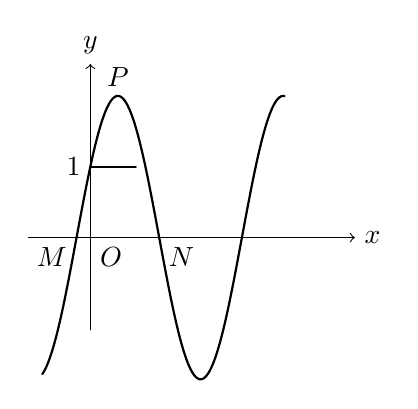
\begin{tikzpicture}[line cap=round,line join=round,x=1.05cm,y=0.9cm]
  \draw[->] (-0.75,0)--(3.2,0) node[right] {$x$};
  \draw[->] (0,-1.3)--(0,2.45) node[above] {$y$};
  \draw[thick] plot[domain=-0.58:2.35,samples=140] (\x,{2*sin(180*\x+30)});
  \draw[thick] (0,1)--(0.55,1);
  \node[left] at (0,1) {$1$};
  \node[above] at (1/3,2) {$P$};
  \node[below left] at (-1/6,0) {$M$};
  \node[below right] at (5/6,0) {$N$};
  \node[below right] at (0,0) {$O$};
\end{tikzpicture}
